\section{Probability theory recap}
Probability theory is a branch of mathematics concerning numerical descriptions
of how likely an event is to occur. Formalised by Andrey Kolmogorov in 1933.
\cite{kolmogorov2018foundations} He formalised the modern interpretation of 
probability theory. The axioms from this publication is:

\medskip

\textbf{The First Axiom}: The Probability of an event $E$ is a non-negative real
number.

\begin{equation}
    P(E) \in \mathbb{R}, P(E) \geq 0, \quad \forall E \in F 
\end{equation}

where $F$ is the event space.

\medskip

\textbf{The Second Axiom}: The Probability of at least one element occuring in
the sample space is $1$

\begin{equation}
    P(\Omega) = 1
\end{equation}

\medskip

\textbf{The Third Axiom}: The probability of the union of disjoint sets is equal
to the sum of the probabilities of the disjoint sets.

\begin{equation}
    P\left(\bigcup_{i = 1}^{\infty} E_i \right) = \sum_{i = 1}^{\infty} P(E_i)
\end{equation}

\section{Conditional Probability Recap}

\begin{equation*}
P(A \mid B) = \frac{P(A \cap  B)}{P(B)}
\end{equation*}

This is read as: Probability of event A given B. 

\section{Bayes Theorem}

Bayes theorem is derived from the definition of codnitional 
probability. Given that

\begin{equation*}
    P(A \cap B) = P(B \cap A)
\end{equation*}

Since the intersection operator does not care about order. We can rearrange
equation and get

\begin{equation*}
    P(A \cap B) = P(A \mid B)P(B) = P(B \mid A)P(A)
\end{equation*}

and we can substitute $P(A \cap B)$ with the equation above and get:

\begin{theo}[]{theo:theo91}
\label{eq:bayes}
\[
P(A \mid B) = \frac{P(B \mid A) P(A)}{P(B)}
\]
\end{theo}

\section{Bayes Theorem for Continuous Values}

We need to assume that the values we are interested in have a Gaussian distribution.
\begin{itemize}
    \item Find the mean $\mu$
    \item Find the variance $\sigma^2$
    \item Use the Gaussian distribution to calculate the probability $P(A)$
\end{itemize}
\medskip

For conditional probabilities:
\begin{itemize}
    \item Find the mean $\mu_B$ for only the condition $B$
    \item Find the variance $\sigma^2_B$ for only the condition $B$
    \item Use the Gaussian distribution to calculate the conditional probability $P(A|B)$
\end{itemize}
\medskip

For inequalities, we need to integrate the Gaussian density (preferably by computing the standard Gaussian density first).

\section{Bayesian Classifiers}
\subsection{Goal}
Given a record with attributes $(A_1, A_2, \cdots, A_n)$, the goal of the bayesian classifier is th predict the class $C$.
Specifically, we want the classifier to fint the value of $C$ that maximizes $P(C|A_1, A_2, \cdots, A_n)$.

\subsection{Approach}
\begin{enumerate}
    \item Compute the posterior probability for all values of $C$ based on Bayes theorem.
    \item Choose the value of $C$ that maximizes the posterior probability.
    \begin{itemize}
        \item This is equivalent to choosing the value of $C$ \\ that maximizes $P(A_1, A_2, \cdots, A_n | C) P(C)$, \\ because the denominators are equal
    \end{itemize}
\end{enumerate}
\medskip

Computing $P(A_1, A_2, \cdots, A_n | C) P(C)$ is done as such:
\begin{enumerate}
    \item Assume independence among attributes $A_i$ when the class is given:
    \begin{itemize}
        \item $P(A_1, A_2, \cdots, A_n | C) = P(A_1|C_j) P(A_2|C_j) \cdots P(A_n|C_j)$ 
    \end{itemize}
    \item Estimate $P(A_i|C_j)$ for all $A_i$ and $C_j$
    \item The new point is classified to $C_j$ if $P(C_j)\prod P(A_i|C_j)$ is maximal
\end{enumerate}

\subsection{Estimating Probabilities from Data}
For continuous attributes:
\begin{enumerate}
    \item Discretize the range into bins:
    \begin{itemize}
        \item One ordinal attribute per bin
        \item Violates independence assumption
    \end{itemize}
    \item Two-way split
    \begin{itemize}
        \item Choose only one of the two splits as a new attribute
    \end{itemize}
    \item Probability density estimation
    \begin{itemize}
        \item Assume that the attribute follows a normal distribution
        \item Estimate the mean and the variance
        \item Estimate the conditional probability $P(A_i|C)$ from the known distribution
    \end{itemize}
\end{enumerate}

\bigskip
\begin{figure}[H]
\centering
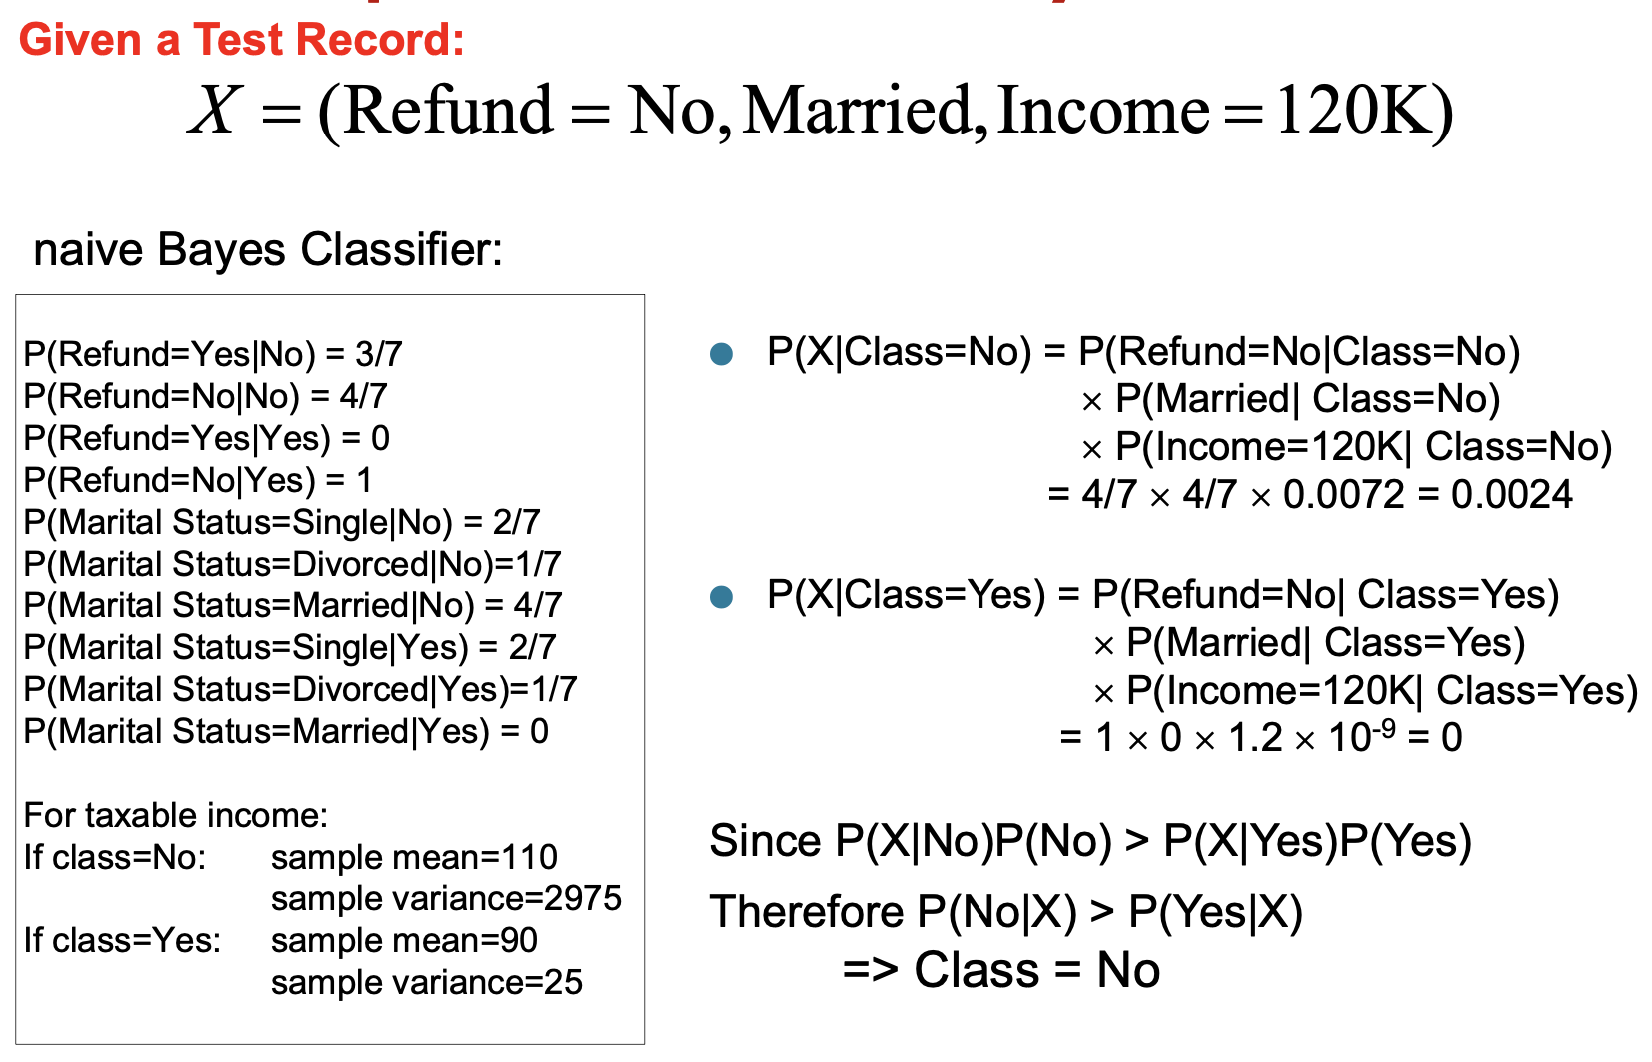
\includegraphics[scale=0.4]{figures/prob_est_data.png}
\caption{Example of deciding class}
\end{figure}

\subsection{Naive Bayes Classifier problems}
In the previous figure, one of the conditional probabilities is zero, meaning that the entire expression becomes zero.
This is often an effect of having an incomplete training set. This means that the class, given the conditional probability, will never be chosen.

This can be "fixed" by using some type of smoothing:
\begin{itemize}
    \item Original: $P(A_i|C) = \frac{N_{ic}}{N_c}$
    \item Laplace: $P(A_i|C) = \frac{N_{ic}+1}{N_c+c}$
    \item m-estimate: $P(A_i|C) = \frac{N_{ic}+mp}{N_c+m}$
\end{itemize}

Where $c =$ number of classes, $p =$ prior probability, and $m =$ own parameter.

\section{Bayesian Belief Network (BBN)}
\begin{itemize}
    \item Conditional independence assumption is not always practical.
    \item A Bayesian belief network provides a graphical representation of dependencies.
    \begin{itemize}
        \item A directed acyclic graph (dag) encoding the dependence relationships among a set of variables.
        \item A probability table associating each node to its immediate parent node.
    \end{itemize}
    \item Calculating the probability of a variable, which is dependent on some other variables, can often be simplified to only depend on the direct parent(s).
\end{itemize}

\section{Summary of Naive Bayes}
\begin{itemize}
    \item Robust to isolated noise points.
    \item Handle missing values by ignoring the instance during probability estimate calculations.
    \item Robust to irrelevant attributes.
    \item Independence assumption may not hold for some attributes.
    \begin{itemize}
        \item Use other techniques such as Bayesian Belief Networks (BBN).
    \end{itemize}
\end{itemize}
